\documentclass[11pt,preprint]{aastex}
 %\documentclass[12pt]{emulateapj}
\usepackage[margin= 1.0in]{geometry}    % See geometry.pdf to learn the layout options. There are lots.
\geometry{letterpaper} % or letter or a5paper or ... etc
\usepackage{float}
\usepackage{amssymb,amsmath}
\usepackage[]{epsfig,graphicx}
\usepackage{color}
\usepackage{verbatim}
\DeclareGraphicsRule{.tif}{png}{.jpg}{`convert Num1 `dirname Num1`/`basename Num1 .tif`.jpg}
\newcommand{\units}[1]{\ensuremath{\, \mathrm{#1}}}
\usepackage{enumitem}
\usepackage{natbib}
\newcommand{\degree}{\ensuremath{^\circ}}
\usepackage[maxfloats=25]{morefloats}
\usepackage[normalem]{ulem}
\usepackage{hyperref}
\usepackage{ amssymb }
\newcommand{\TRANSPOSE}{\ensuremath{T}}

\bibliographystyle{apalike}


\begin{document}
\title{Music Recommendation System Using the Million Song Dataset}

 \author{Jordan Rosenblum, Justin Law \& Erin Grand}
 \affil{Data Science Institute, Columbia University, New York, NY 10027}
 
\date{\today}             

\begin{abstract}
We attempt to build a recommendation system for a subset of the Million Song Dataset. We explore various algorithms including matrix factorization, user-based collaborative filtering, and item-based collaborative filtering. In each case we recommend the top 500 songs that our algorithm returns to each user and compare against the testing set of what the user actually listened to. Matrix factorization gives the worst results, only slightly above the popularity baseline, while artist-based popularity and user-based and item-based collaborative filtering methods yield better results.
\end{abstract}

\tableofcontents

\section{Introduction}
In the online world, recommendation systems are becoming increasingly important in various industries including retail, entertainment, and even dating. 
Because of their popularity and usefulness, there are numerous incentives to implement a good recommendation system. 
In the music industry, companies use recommendation systems to provide a better service to their listeners. 
With the music industry shifting away from a more traditional distribution model of physical CDs or records, 
having an efficient and well performing recommendation system is very important. 

In building a recommendation system, we had to take into account various trade-offs in the type of models we chose to fit. For example, some methods take more information about the user and the song into account (i.e. content-based) while others use a collaborative filtering approach without taking into account user or song characteristics such as age, genre, location, etc. In this paper, we focus on collaborative filtering methods.
There is no set similarity measure between two songs, as evident by the fact that songs by the same artist are often very different. As such, there are many different types of algorithms to explore. 

For our project, we explored various song recommendation systems algorithms such as popularity recommendations, artist based recommendations, matrix factorization, and user and item based similarity measures.  
% memory based collaborative filtering

\subsection{Data and Statistics}
The main source of data for this project was the Million Song Data Set (MSD)  \citep{Bertin-Mahieux2011}. We used the sample data set from the Kaggle competition which contains tuples of user id, song id, and play count. We also used data which links songs to artists through track ids. The links to these datasets can be found in the Appendix.

The sample data set had $110000$ users, $163206$ songs, and the number of play counts for each user and song pair. The statistics are summarized in Table \ref{tab:stats}:

\begin{table}[h]
\begin{center}
\begin{tabular}{lll}
\hline
Measurement & Plays Across Songs & Plays Across Users \\
\hline
Count &  163206 & 110000 \\
Mean  &     8.890194 & 13.190300  \\
Std      &    46.780258 & 8.070827 \\
Min      &    1.0  & 5.0  \\
Max     &   5043 &  53 \\
\end{tabular}
\caption{Basic summary statistics for the full data set.}\label{tab:stats}
\end{center}
\end{table}

It is also easy to see in the below chart that the majority of the songs are listened to by very few users so we can decrease the number of songs in our subset but not lose all of the play count. 

\begin{figure}[htbp] %  figure placement: here, top, bottom, or page
   \centering
   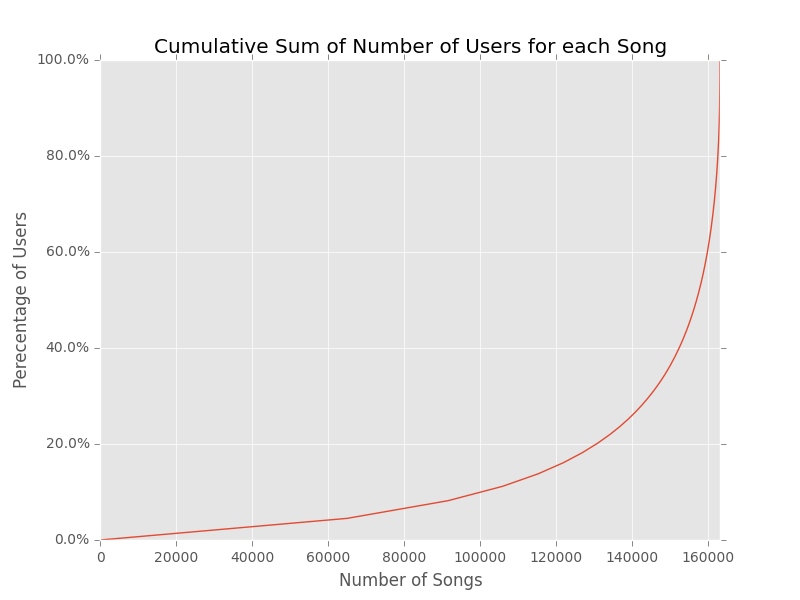
\includegraphics[width=4in]{../plots/final/cumsum-songs.png} 
   \caption{Percentage of users accounted for versus songs with increasing number of plays.}
   \label{fig:t}
\end{figure}

The scale of the data was too large to explore on our computers, so we subset the data down to a size easily handled by an average laptop. 

We choose to subset the data to users who have listened to more than 27 songs and songs which were listened to by more than 22 users. This resulted in a dataset which was 10\% the size of the original. The sparsity of the data was .0016, meaning that we only had play counts for 0.16\% of the user, song pairs (i.e. not all users listen to all songs). Despite subsetting the data, though, we are still dealing with a matrix of $8130$ users by $11861$ songs, so some of our algorithms will take a fair amount of time to run.

%\begin{figure}[htbp] %  figure placement: here, top, bottom, or page
%   \centering
%   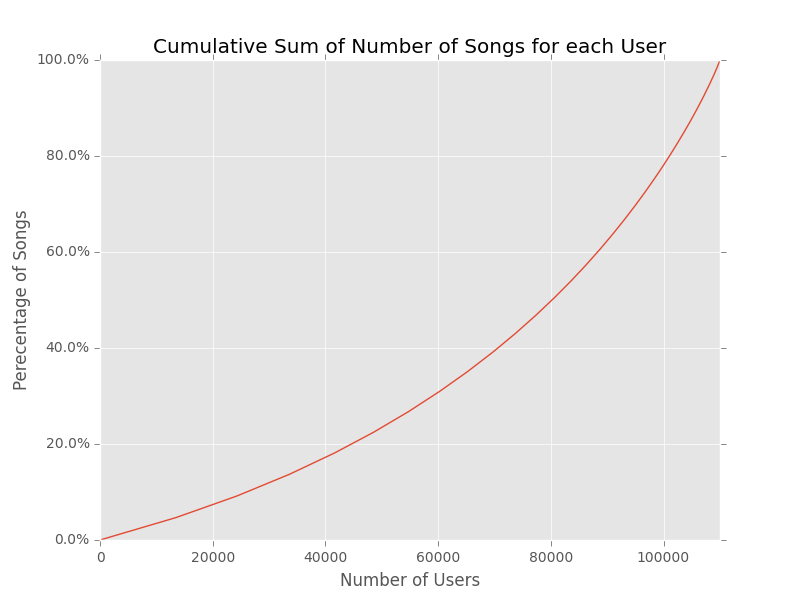
\includegraphics[width=4in]{../plots/final/cumsum-users.png} 
%   \caption{Percentage of songs accounted for versus users with increasing number of plays.}
%   \label{fig:t}
%\end{figure}


%\begin{figure}[htbp] %  figure placement: here, top, bottom, or page
%   \centering
%   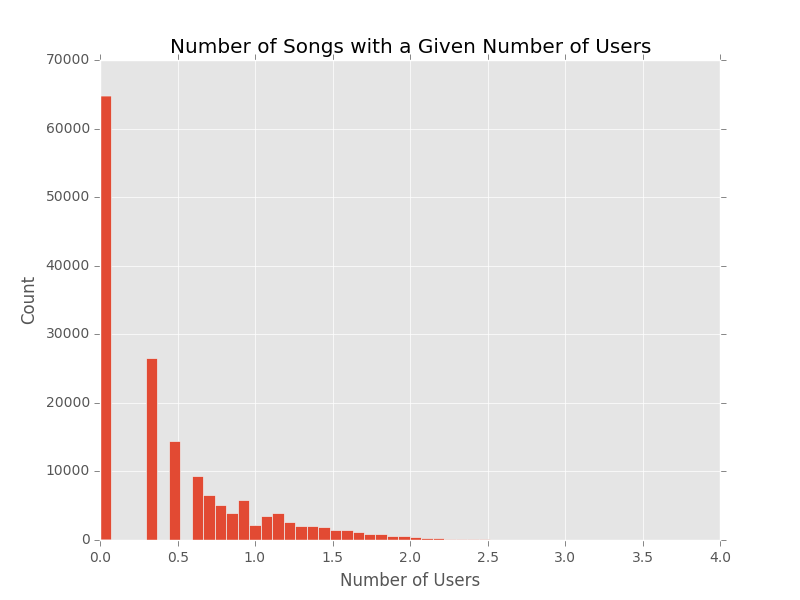
\includegraphics[width=4in]{../plots/final/hist-song.png} 
%   \caption{ }
%   \label{fig:t}
%\end{figure}
%
%
%\begin{figure}[htbp] %  figure placement: here, top, bottom, or page
%   \centering
%   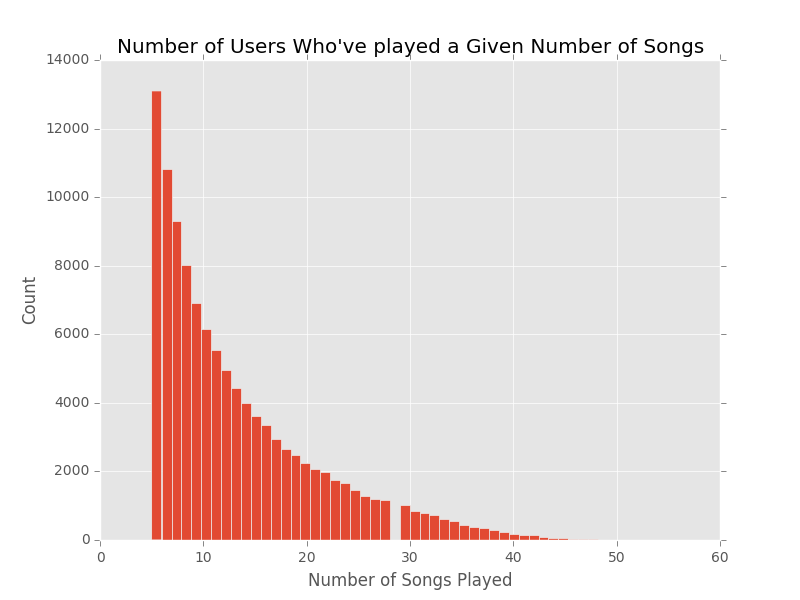
\includegraphics[width=4in]{../plots/final/hist_user_song_count.png} 
%   \caption{ }
%   \label{fig:t}
%\end{figure}


\subsection{Data Analysis}
In order to perform the analysis, we had to fill in training and testing matrices which contained play counts for user and song pairs. We did a random selection of data elements to split between the training (80\%) and testing (20\%) sets. Next, we implemented various algorithms on the dataset in order to recommend songs to users, including matrix factorization, user-based collaborative filtering, and item-based collaborative filtering.

\subsection{Testing}
We tested our algorithms against each other using a mean average precision 
score for each method.  The mean average precision (MAP) calculation came directly from the Kaggle MSD challenge \citep{McFee:2012:MSD:2187980.2188222}. The score was used to rank the competition entries.

Specifically, we used MAP@500 scores which take into account the first 500 recommendations given to each user. Generally, the score looks at the precision between a list of recommendations for a user and that user's test set. This was done by calculating the average precision at each element in the list of recommended items (i.e. percentage of correct items among first $k$ recommendations) and averaging these for the first 500 recommendations (i.e. for each $k \in \{1, ..., 500\}$, calculate the precision and average them together).
We then averaged the score over all users. Intuitively, the score looks at the percentage of recommendations that were in-line with the test set of songs actually listened to but also takes order into account. So it is preferable to recommend the songs in the user's test set earlier in the list of 500. The MAP score is similar to the AUC of the ROC curve discussed in class except it takes ordering of the recommendations into account, which is an important factor to consider in a recommendation system.

We used two different baseline benchmarks \citep{McFee:2012:MSD:2187980.2188222} to compare our MAP scores against. The first was to simply recommend the top 500 most popular songs to every user. This naive method resulted in a MAP score of 0.0138 (top 500 songs based on number of users who listened to the song) or 0.0126 (top 500 songs based on number of plays the song had). The second method was to first recommend a user the most popular songs of artists the user already had already played (but different songs from that artist). If this did not result in enough recommendations, we would then recommend the overall most popular songs as well at the end (similar to baseline method 1). Although this method is conservative in that it does not go beyond the tastes the user already has in the training set, it resulted in a significant improvement in the MAP score to 0.0448.

\section{Algorithms}

\subsection{Probabilistic Matrix Factorization}
Matrix factorization is a type of collaborative filtering algorithm that can be used to build a recommendation system for users based on user feedback of objects (in this case songs). This allows us to recommend songs to users based on their listening history without the need for content based approaches. 
Training and testing matrices were constructed, of which both have $N_1$ users (rows denoted by $u_i$) and $N_2$ songs (columns denoted by $v_j$). As users have only listened to a fraction of all the songs available, the matrices are sparse, containing zeros in all entries except for those in which a user (a user representing a single row) has listened to. The goal of matrix factorization is to factor the training matrix into the product of two matrices $U$ and $V$.  The matrix $U$ is $N_1 \times d$ and the matrix $V$ is $d \times N_2$. Another goal of matrix factorization is typically to learn a low-rank factorization of the original matrix while restricting the patterns that are generated in the product of the factorized matrices (e.g. if a user likes a song in a specific group of songs, the user may also like other songs in that group of songs). The choice of $d$ can be subjective but $20$ is a common value to start with. In the factorized matrices, the predicted rating will be $\hat{M}_{ij} = u_i^\TRANSPOSE  v_j$
Using a coordinate ascent algorithm over 100 iterations, each row ($u_i$) and column ($v_j$) of the training matrix is then updated (equations \ref{eq1} and \ref{eq2}) in order to maximize the log joint likelihood (equation \ref{eq3}).

\begin{equation}
u_i = \left( \lambda\sigma^2 I + \sum_{j \in \Omega_{u_i}} v_j v_j^\TRANSPOSE \right)^{-1}\left(\sum_{j \in \Omega_{u_i}} M_{ij} v_{j} \right)
\label{eq1}
\end{equation}

\begin{equation}
v_j = \left( \lambda\sigma^2 I + \sum_{i \in \Omega_{v_j}} u_i u_i^\TRANSPOSE  \right)^{-1}\left(\sum_{i \in \Omega_{v_j}} M_{ij} u_{i} \right)
\label{eq2}
\end{equation}

\begin{equation}
\mathcal{L} = \sum_{(i,j) \in \Omega} \frac{1}{2\sigma^2} {|| M_{ij} - u_i^\TRANSPOSE  v_j||}^2 - \sum_{i=1}^{N_1} \frac{\lambda}{2} ||u_i^2 || - \sum_{i=1}^{N_2} \frac{\lambda}{2} ||v_j^2 || + \text{constant}
\label{eq3} 
\end{equation}

\emph{Note: $\lambda = 10$ was used and $\Omega$ is the set of all indices in the matrix which have an observation.}

There are several hyper-parameters that can be tweaked in order to achieve a better MAP result using matrix factorization. The main ones that we varied were the variance, the rank $d$ of the factorization, and the number of iterations. As the project was being done using Python and the main computational package (\emph{scikit-learn}) did not have probabilistic matrix factorization functions, we decided to apply the algorithm that we wrote ourselves for a different class \citep{koren2009matrix}. 
 
After testing various values of the parameters, it was soon discovered that matrix factorization results were significantly below the popularity baseline and changing the hyper-parameters around did not help much. The best MAP value of 0.0038 was achieved using a high rank $d$ of 80 over 100 iterations with a variance of 1.0. The log joint likelihood chart can be used to verify that the probabilistic matrix factorization algorithm is running properly in that the values are monotonically decreasing which corresponds to a decreasing training error. The plot shows that there is more room for improvement of the training error, but the MAP plot that was taken from the same run shows that there is only a marginal difference in terms of improving the MAP score after the initial 5 iterations. Due to this result, further exploration of the probabilistic matrix factorization algorithm was limited to 30 iterations to reduce computational time. 

\begin{figure}[htbp] %  figure placement: here, top, bottom, or page
   \centering
   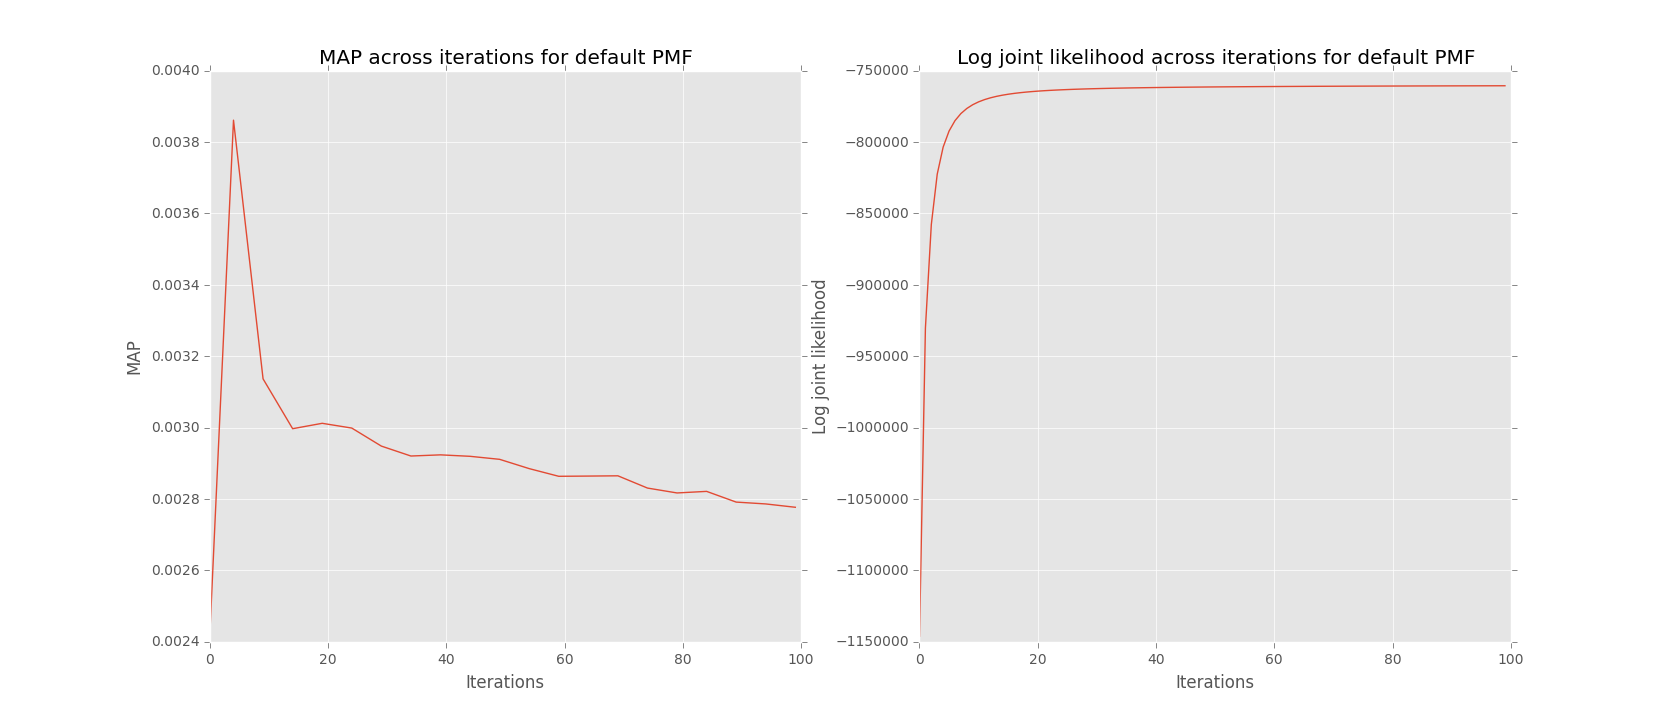
\includegraphics[width=6in]{../plots/final/defaultPMF.png} 
   \caption{MAP values and log joint likelihood values for PMF using default playcount values with $\sigma^2 = 1.0$ and $d = 80$}
   \label{defaultPMF}
\end{figure}
 
One explanation for the very low MAP scores using PMF was that the number of plays that were used are different from what PMF is typically used for which is bounded ratings. Using implicit user feedback (number of plays) instead of explicit user feedback (ratings) has been found in literature to create various issues. One of the main issues is that implicit feedback is inherently noisy and does not measure negative feedback. Users may have played a song to simply find out that they dislike the song. The other main issue is that the exact number of plays could have a significantly different meaning across different users. For example, an avid user who has played a song five times could have a different meaning as compared to a user that has at most only played songs five times.
 
In order to tackle the issue of using implicit user feedback, we tried four different scaling schemas independently. These included normalizing user play counts by the total number of plays for the user, normalizing song play counts by the total number of plays for the song, making the data binary (changing all non-zero play counts to 1), and  applying tf-idf. While testing out these schemas, we continued to vary the hyper-parameters (i.e. $d$ and variance) in order to determine if they changed the MAP results significantly. 
 
From the experiments, it was found that the rank $d$ did not contribute significantly to the MAP values especially in settings where the MAP values were close to the baseline. Higher variance values were found to actually significantly increase the MAP values. In terms of scaling schemas, making the data binary produced the best result, with the second best being normalizing the data against the total number of plays for each user. Perhaps it can be said that using number of plays introduces more noise than simply considering if the user has played the song or not. Interestingly enough, normalizing the data against total number of plays for each song performed the worst and this most likely relates to the fact that number of plays is more meaningful relative to each user rather than to each song.
 
\begin{figure}[htbp] %  figure placement: here, top, bottom, or page
   \centering
   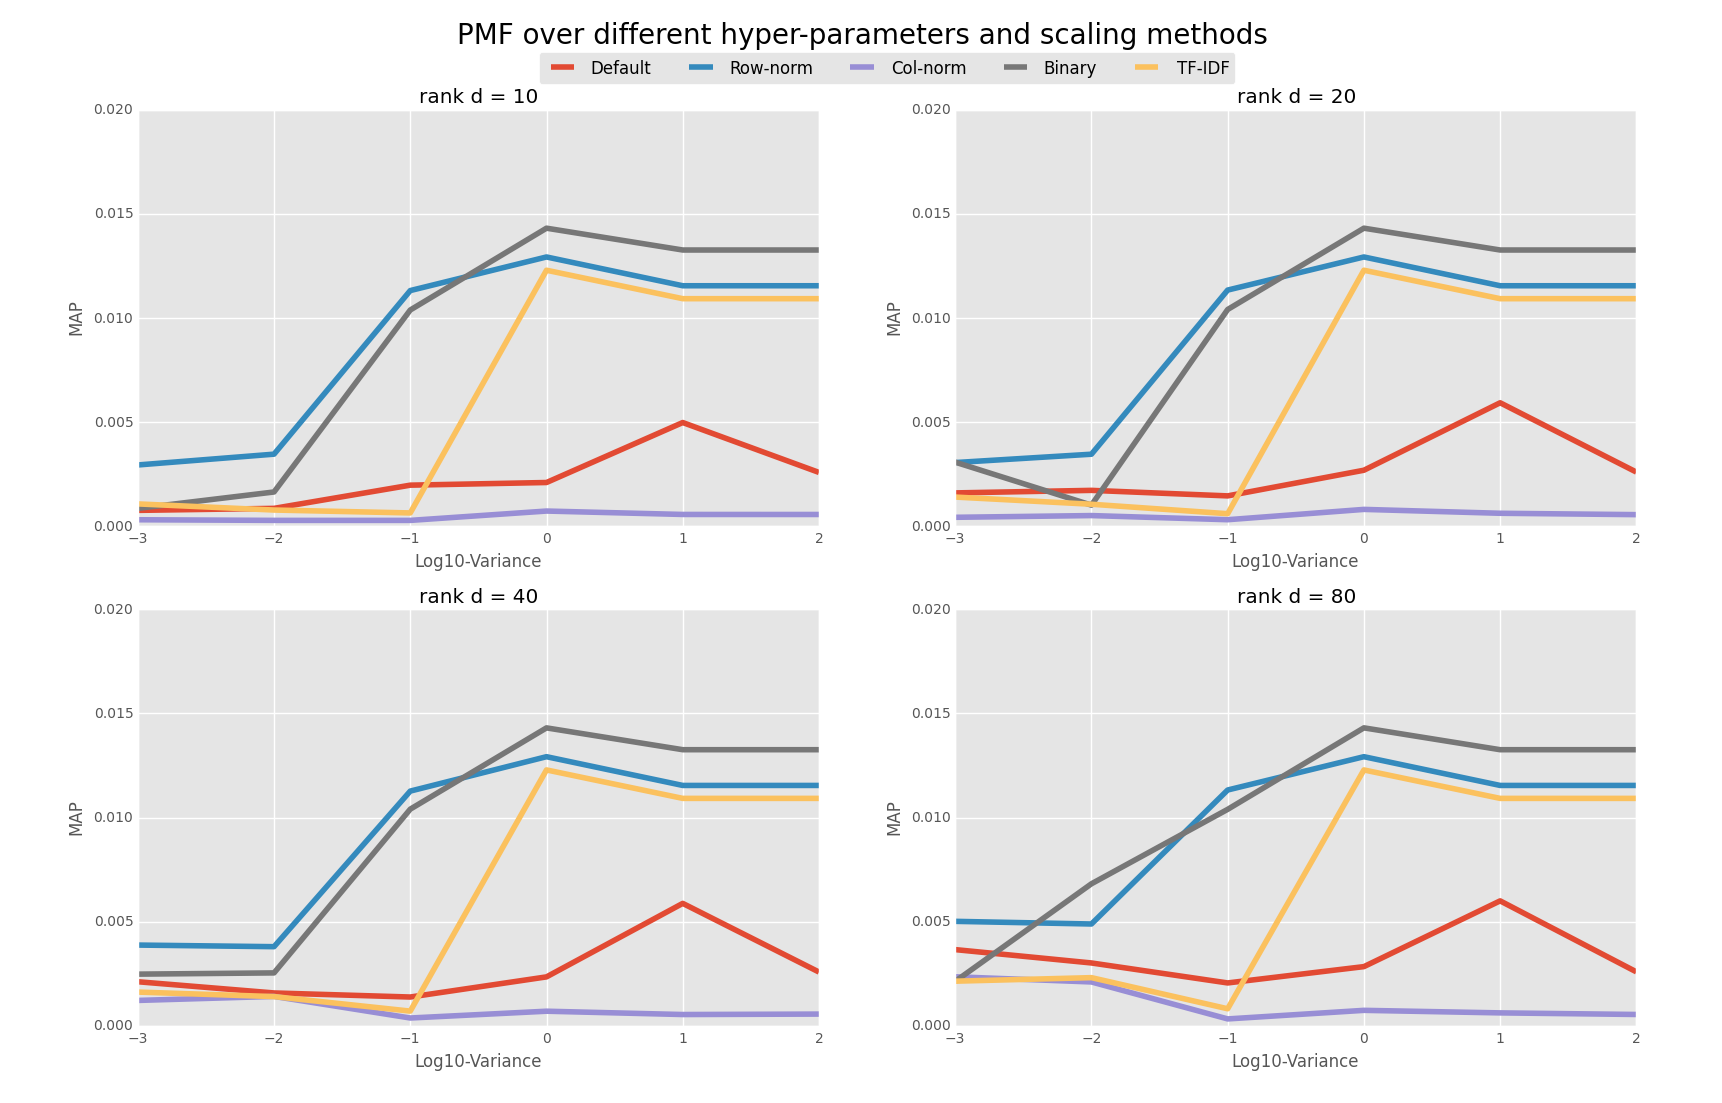
\includegraphics[width=6in]{../plots/final/PMF.png} 
   \caption{MAP values for different scaling methods and hyperparameters after 30 iterations}
   \label{PMF}
\end{figure}
 
Regardless, the best result achieved for PMF in the end was 0.0143, which was only slightly above the popularity baseline. Based on literature review, we have found that this is better or in line with what others have achieved with using PMF on play counts. Nevertheless, this indicates that PMF is not suitable for the MSD dataset and this can be attributed to the implicit feedback issue or simply to the fact that the dataset is too sparse. However, it is still possible to apply matrix factorization techniques to this dataset through using metadata and this has been demonstrated to be viable by \citet{liangcodebook} which achieved MAP values exceeding 0.1.  

\citep{hu2008collaborative}





%
%\begin{figure}[ht]
%\begin{minipage}[b]{0.45\linewidth}
%\centering
%\includegraphics[width=\textwidth]{h845BuzFO9CNgAAAABJRU5ErkJggg==.png}
%\caption{default}
%\label{fig:figure1}
%\end{minipage}
%\hspace{0.5cm}
%\begin{minipage}[b]{0.45\linewidth}
%\centering
%\includegraphics[width=\textwidth]{C9LAAAAABJRU5ErkJggg==.png}
%\caption{default}
%\label{fig:figure2}
%\end{minipage}
%\end{figure}

\subsection{User Based and Item Based Collaborative Filtering}
%\subsubsection{Intro to Memory-Based Collaborative Filtering}
A simpler set of methods for determining which songs to recommend to individual users is by using user- or item/song- based similarity (both also considered collaborative filtering). These only consider whether or not a user listened to a song and does not take into account the play count. Similarity scores between users (i.e. user-based) and songs (i.e. item-based) were calculated using cosine similarity \citep{aiolli2013preliminary, li2012million}. Intuitively, they work by recommending users songs that other similar users like (user-based) or by recommending songs which are similar to the songs the user has already listened to (item-based). The downside to this method is the computational complexity. Given the quadratic runtime of these algorithms, they are more difficult to scale to a larger dataset. As for storage requirements, we will have to store all pairs of similarity scores for users in the case of user-based and songs in the case of item-based. The details are described below.

\subsubsection{User-Based Collaborative Filtering}
For user-based recommendation, we first calculated the similarity score between every pair of users, $u$ and $v$, using equation \ref{eq:item}:

\begin{equation}
sim(u,v) = \frac{\text{\# common items}(u, v)}{{\text{\# items}(u)}^{1/2} \times {\text{\# items}(v)}^{1/2}}
\label{eq:item}
\end{equation}

Then, for each user, we looked at each song in the dataset and found all other users who have listened to that song. Next, we added up the similarity score of each of those users, $v$, with the original user, $u$, and got the weight for a particular song, $i$:  

$$w_i = \sum_{v \in V} sim(u, v)$$

The sum is a proxy for how likely the user is to like that particular song. We went through that process for all songs and recommended the user the top 500 songs which had the highest scores. This method led to a MAP value of 0.0377.

\subsubsection{Item-Based Collaborative Filtering}
For item-based recommendation, which turned out to be our best algorithm in terms of a MAP value, we first calculated the similarity score between every pair of songs, $i$ and $j$, using equation \ref{eq:user} and saved the most similar songs to each song in the process:

\begin{equation}
sim(i,j) = \frac{\text{\# common users}(i, j)}{{\text{\# items}(i)}^{1/2} \times {\text{\# items}(j)}^{1/2}}
\label{eq:user}
\end{equation}

Then, for each user, we found all the songs listened to. Next, we got the most similar songs to each of those songs listened to by the user. If the same similar songs came up multiple times, we added the weights together. In other words, for each song, $b$, that was found to be similar to one of the songs, $a$, that the user listened to, we calculated the score for that song, $b$:

$$w_b = \sum_{a \in A} sim(a, b)$$

Lastly, we sorted the songs by scores and recommended the user the top 500 songs which had the highest scores. This method led to a MAP value of 0.0479.


%\subsection{Artist Based Recommendation}



\section{Results}
After comparing the various algorithms, the simpler models gave us the best results. Our most complicated model, matrix factorization, gave us results barely above the popularity baseline. On the other hand, simply recommending users songs by artists they have already listened to (the artist-based popularity baseline) resulted in a significantly better recommendation system. Our song-based collaborative filtering technique produced the best results despite being a relatively simple algorithm as compared to matrix factorization. Our final results for each technique employed are summarized in the table below. 

\begin{table}[h]
\begin{center}
\begin{tabular}{lc}
\hline
\bf{Algorithm} &  \bf{MAP score}\\ \hline
Item Based  CF  &  0.0479 \\ 
Artist Based Popularity Baseline  & 0.0448    \\ 
User Based  CF  &  0.0377 \\ 
Matrix Factorization  &   0.0143  \\ 
Top 500 Songs by Count  Baseline &  0.0138  \\ 
Top 500 Songs by Plays  Baseline &  0.0126  \\ 
\end{tabular}
\caption{Final MAP results across various algorithms.}\label{tab:stats}
\end{center}
\end{table}

\section{Conclusion}
Apart from the algorithms discussed above, we also explored building a recommendation system based on K-Means Clustering (by both user and song) and Non-Negative Matrix Factorization (NMF). In the end, both of these methods yielded worse results as compared to Probabalistic Matrix Factorization so we decided not to explore them further. Next steps include incorporating tags and metadata present in the dataset (e.g. year, genre, and audio metadata). It would also be useful to expand the size of the subset and distribute the workload to multiple machines so that more data could be analyzed.

%To Reference a paper: 

%The Million Song Dataset Challenge: \citep{McFee:2012:MSD:2187980.2188222} \\
%Million Song Dataset Recommendation Project Report: \citep{li2012million} \\
%codebook-based scalable music tagging with poisson matrix factorization: \citep{liangcodebook} \\
%Matrix Factorization Techniques for Recommender Systems: \citep{koren2009matrix} \\
%A Preliminary Study on a Recommender System for the Million Songs Dataset Challenge: \citep{aiolli2013preliminary} \\



\bibliography{msdref}

\small{
\section{Appendix}

\begin{itemize}

  \item Link to our github repository: \url{https://github.com/eringrand/musicanalysis}
  \item The MSD Kaggle challenge: \url{https://www.kaggle.com/c/msdchallenge}
  \item The user, song, play count dataset: \url{https://www.kaggle.com/c/msdchallenge/download/kaggle_visible_evaluation_triplets.zip}
  \item Data to link songs to artists through track ids: \url{http://labrosa.ee.columbia.edu/millionsong/sites/default/files/AdditionalFiles/track_metadata.db}

\end{itemize}
}

\end{document} 
